\mcchap{Il portale Covid19-Italy}{cap:portale}
Con il patrocinio dell’Università degli studi dell’Insubria è stato ideato il portale Covid 19-Italy.it\footnote{https://covid19-italy.it}, un sito che permette di visualizzare i dati aggregati e ufficiali sull’andamento della pandemia regione per regione e a livello nazionale, attraverso grafici e confronti.
Sulla pagina principale del sito sono presenti 4 card, che permettono di accedere alle seguenti pagine:
\begin{itemize}
\item \emph{Italy R0(t) Indices} permette di accedere alla pagina sulla stima degli indici di riproduzione R0(t) usando il metodo Wallinga and Teunis ,a livello nazionale,  regioni e per provincia.
\item \emph{Italy dashboard} visualizza il monitoraggio del Covid-19 in Italia, attraverso 9 diversi grafici, sempre aggiornati con la pubblicazione di nuovi dati;
\item \emph{Lombardy dashboard} visualizza l’andamento nella pandemia in dettaglio nella regione Lombardia;
\item \emph{Region dashboard} mostra l’andamento della pandemia in una regione italiana a scelta.
\end{itemize}
\begin{figure}[htp]
    \centering
    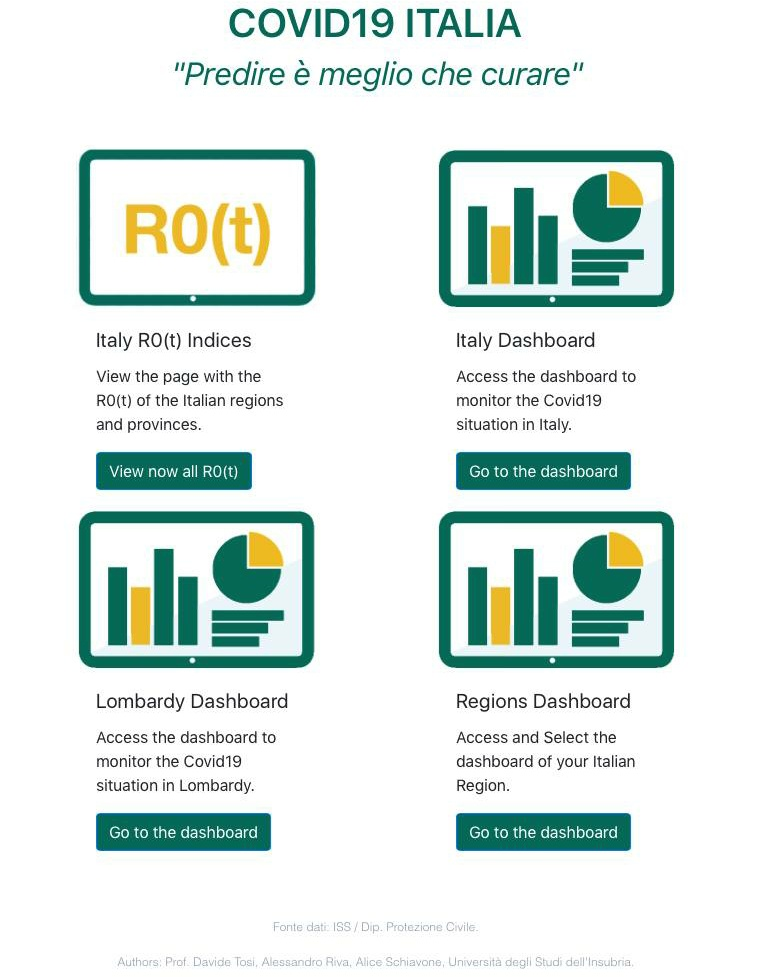
\includegraphics[width=14cm]{covid_19_italy_compact}
    \caption{Pagina principale del sito}
    \label{fig:home_page}
\end{figure}

